\section{State-dependent Poisson Process}

\begin{frame}{State-dependent Poisson Process} 
    This model, introduced by \textit{Fulgenzi, Melatos \& Hughes (2017)}, provides an alternative framework for pulsar glitches.

    \vspace{0.4cm}
    \textbf{Core Idea:}
    \begin{itemize}
        \item Between glitches, the stress $X(t)$ increases \textbf{deterministically}.
        \item Glitches do not occur at a fixed threshold. Instead, the \textbf{instantaneous glitch rate, $\lambda(X)$}, increases as the stress $X(t)$ grows.
    \end{itemize}

    \vspace{0.2cm}
    This means glitches become more likely as the system approaches a critical stress level, but can occur at any time.
\end{frame}

\begin{frame}{SDP: The Master Equation}
    The SDP model is a \textbf{Continuous-Time Markov Chain (CTMC)} where the "state" is the continuous stress level $X$.
    
    The evolution of $p(x, t)$ is governed by the \textbf{Master Equation}:
    \begin{equation}
    X(t) = X(0) + f \cdot t - \sum_{i=1}^{N(t)} \Delta X^{(i)}
    \end{equation}
    \vspace{-1em}
    \begin{itemize}
        \item $f$: Deterministic stress loading rate ($\dot{X}_{sd}$).
        \item $\sum \Delta X^{(i)}$: Sum of stochastic stress drops from glitches.
    \end{itemize}

    \vspace{0.2cm}

    The \textbf{glitch rate} $\lambda(X)$ depends on the current stress:
    \begin{equation}
    \lambda(X) = \frac{\alpha \cdot f}{X_{peak} - X}
    \end{equation}
    \vspace{-1em}
    This rate diverges as $X \to X_{peak}$, making a glitch almost certain.
\end{frame}

\begin{frame}{SDP: How to Sample Glitches?}
    Unlike the step-based Brownian model, the SDP model is \textbf{event-driven}. This simulation method is a form of the \textbf{Gillespie Algorithm} adapted for a time-varying rate.

    {\setlength{\leftmargini}{1em}
    \textbf{Sample Waiting Time ($\Delta t$):}
    
    \begin{itemize}
        \item Given $X_0$, we solve the Gillespie integral $\int_0^{\Delta t} \lambda(X_0 + f \tau) d\tau = -\ln(U)$.
        \item For this model, it yields the analytical solution \cite{FulgenziMelatosHughes2017}:
        \begin{equation}
        \Delta t = \frac{X_c - X_0}{f} \left(1 - U^{f/\alpha}\right), \quad U \sim \text{Uniform}(0,1)
        \end{equation}
    \end{itemize}
    
    \textbf{Sample Glitch Size ($\Delta X_{release}$):}
    \begin{itemize}
        \item The stress just before the glitch is $X_p = X_0 + f \cdot \Delta t$.
        \item The stress drop $\Delta X_{release}$ is then sampled from a distribution $\eta(\Delta X | X_p)$ that is \textbf{conditional} on the pre-glitch stress $X_p$.
    \end{itemize}
    }
\end{frame}

\begin{frame}{SDP: Trajectory}
    The deterministic, linear increase in stress between stochastic glitches results in a characteristic \textbf{sawtooth pattern}.

    \begin{figure}
        \centering
        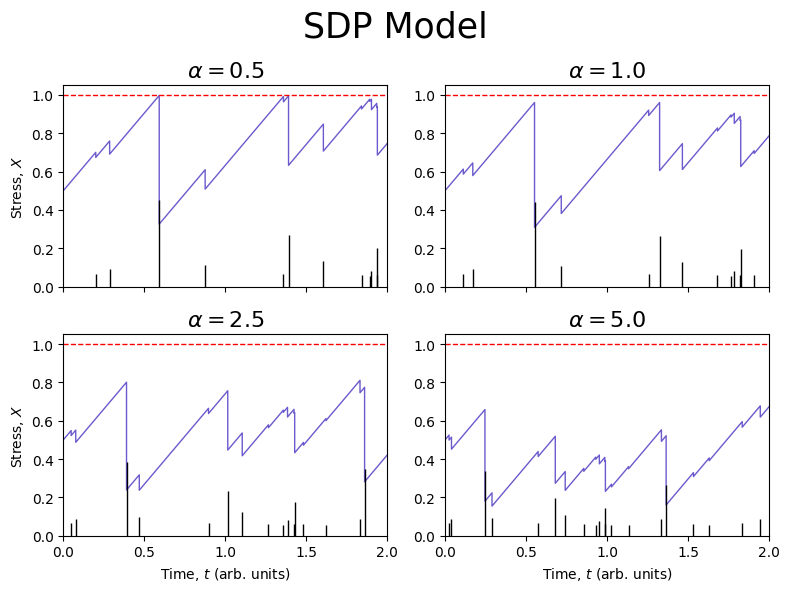
\includegraphics[width=0.75\linewidth,trim=0 0 0 45,clip]{assets/traj_sdp.png}
        \vspace{-1em}
        \caption{A typical stress trajectory for the SDP model. }
    \end{figure}

    Note the linear ramps between random drops.
\end{frame}

\begin{frame}{SDP: Waiting Time Distribution (Power Law)}

    A \textbf{power-law} glitch size distribution generates a \textbf{power-law-like} waiting time. Higher $\alpha$ values lead to a steeper cutoff, reducing the probability of long waiting times and making glitches more regular.

    \begin{figure}
        \centering
        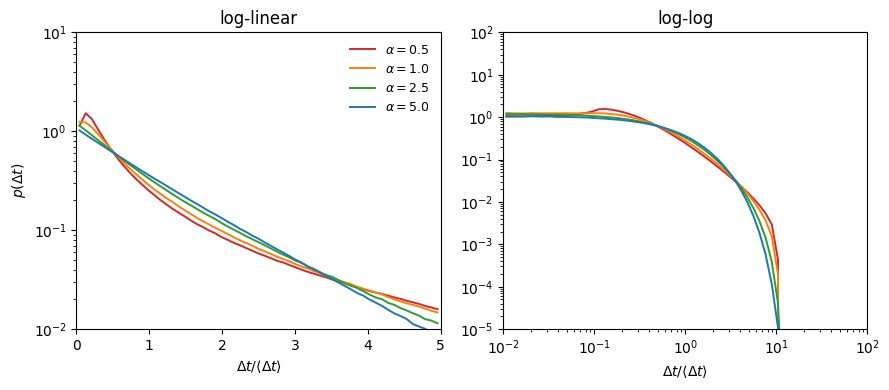
\includegraphics[width=0.85\linewidth]{assets/wtd_powerlaw_sdp.png}
        \vspace{-1em}
        \caption{$p(\Delta t)$ for SDP model, power-law $\eta(\Delta X)$.}
    \end{figure}
\end{frame}

\begin{frame}{SDP: Waiting Time Distribution (Gaussian)}
    \setlength{\leftmargini}{0.5em}
    \small
    \vspace{-0.5em}
    \begin{itemize}
        \item \textbf{High $\alpha$}: $p(\Delta t)$ is exponential-like, characteristic of random, uncorrelated events.
        \item \textbf{Low $\alpha$}: $p(\Delta t)$ is unimodal and narrow, implying predictable, quasi-periodic glitches.
    \end{itemize}

    \vspace{-0.5em}
    \begin{figure}
        \centering
        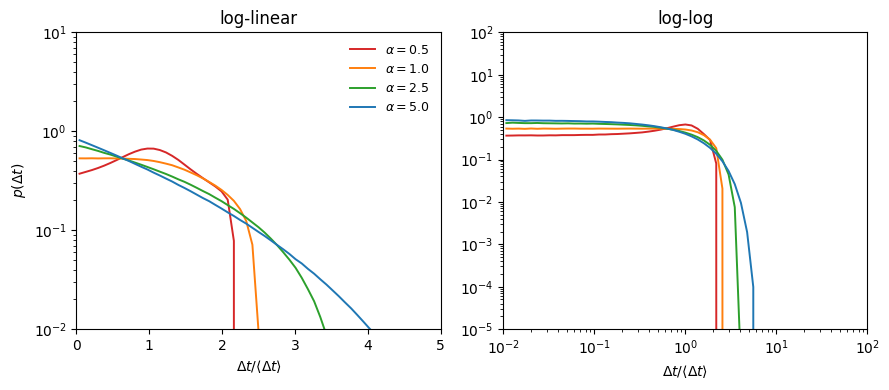
\includegraphics[width=0.85\linewidth]{assets/wtd_gaussian_sdp.png}
        \vspace{-1em}
        \caption{$p(\Delta t)$ for SDP model, Gaussian $\eta(\Delta X)$.}
    \end{figure}
\end{frame}

\begin{frame}{SDP: Waiting Time Distribution (Log-normal)}
    \setlength{\leftmargini}{0.5em}
    \small
    \vspace{-0.5em}
    \begin{itemize}
        \item \textbf{High $\alpha$}: $p(\Delta t)$ is exponential-like, dominated by random glitch triggers.
        \item \textbf{Low $\alpha$}: $p(\Delta t)$ is unimodal and narrow, similar to the Gaussian case.
    \end{itemize}
    
    \vspace{-0.5em}
    \begin{figure}
        \centering
        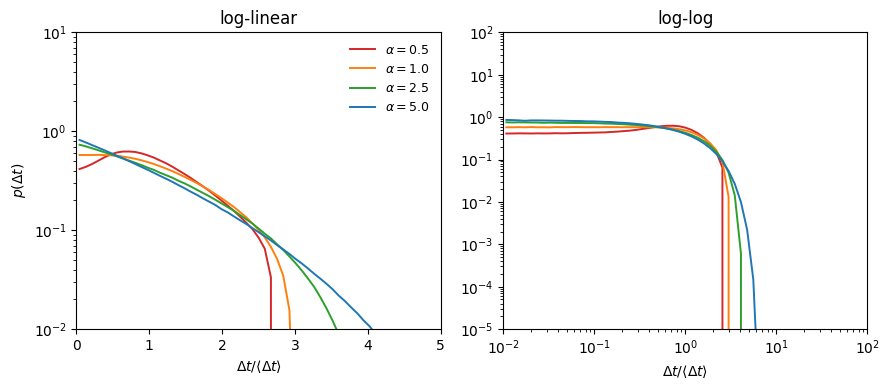
\includegraphics[width=0.85\linewidth]{assets/wtd_lognormal_sdp.png}
        \vspace{-1em}
        \caption{$p(\Delta t)$ for SDP model, Lognormal $\eta(\Delta X)$.}
    \end{figure}
\end{frame}